\section{Applications}
\label{s:numerics}

\begin{figure}%[H]
\centering
%  \begin{tabular}{c c c c c c}
 (a) 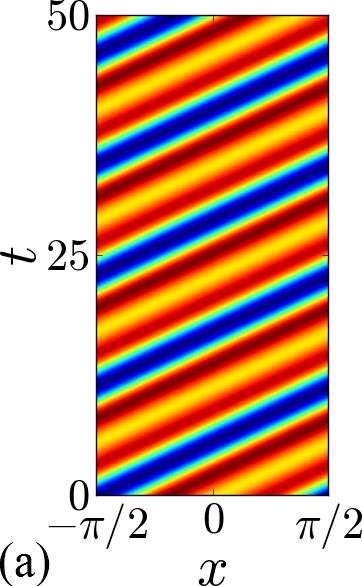
\includegraphics[width=0.12\textwidth]{2modes-conf-reqv} %&
 (b) 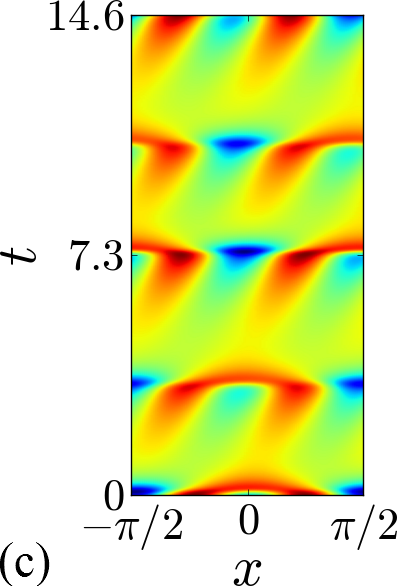
\includegraphics[width=0.12\textwidth]{2modes-conf-rpo} %&
 (c) 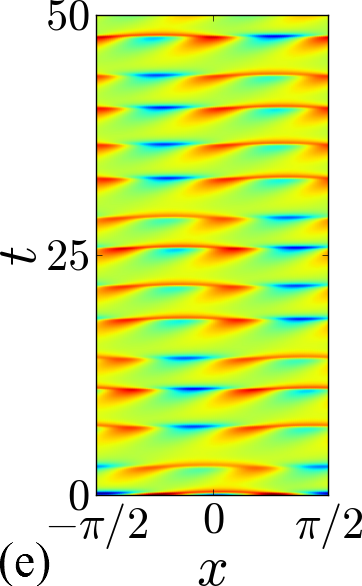
\includegraphics[width=0.12\textwidth]{2modes-conf-ergodic} \\ %&
 (d) 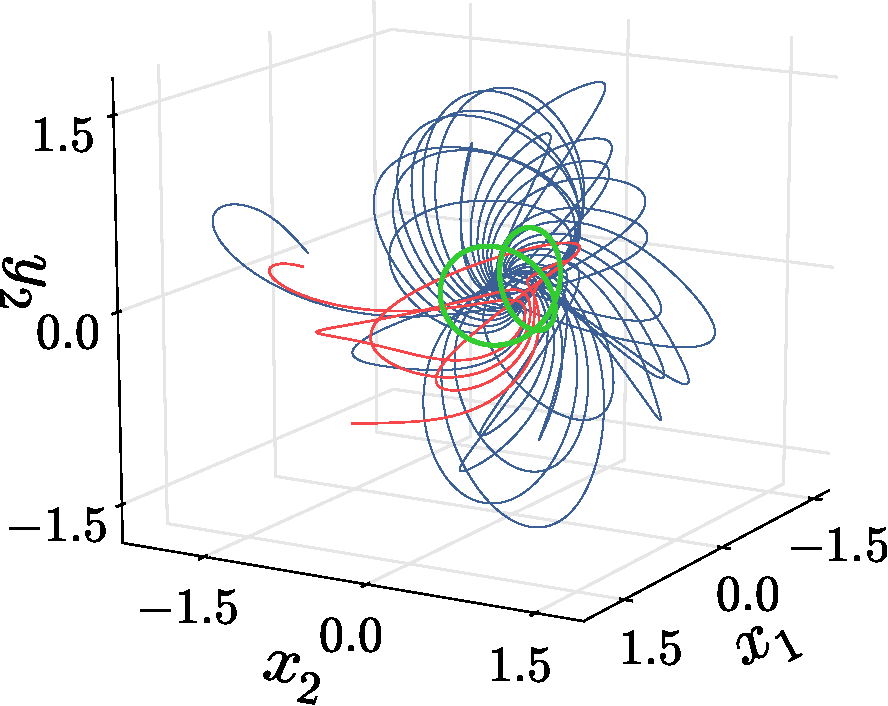
\includegraphics[width=0.45\textwidth]{2modes-ssp} \\ %&
 (e) 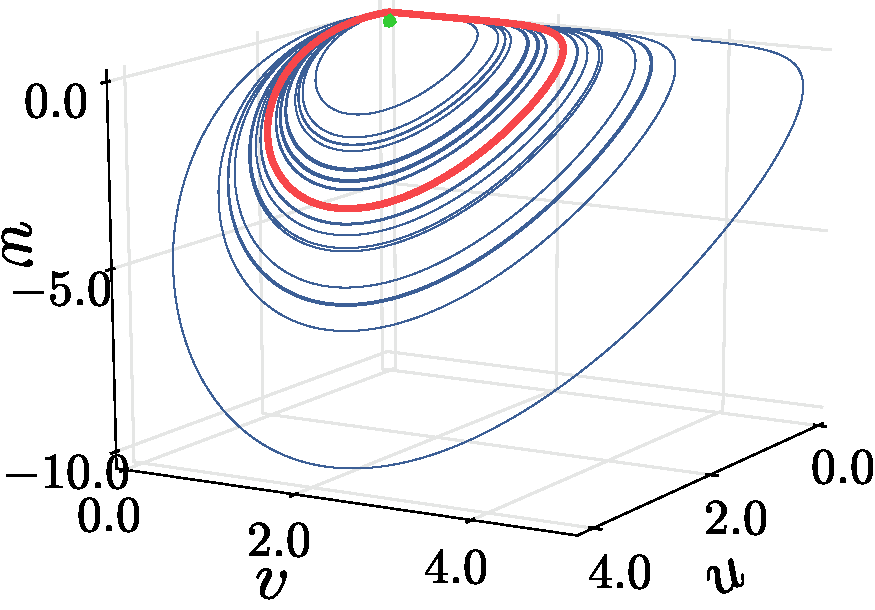
\includegraphics[width=0.21\textwidth]{2modes-invpol} %& 
 (f) 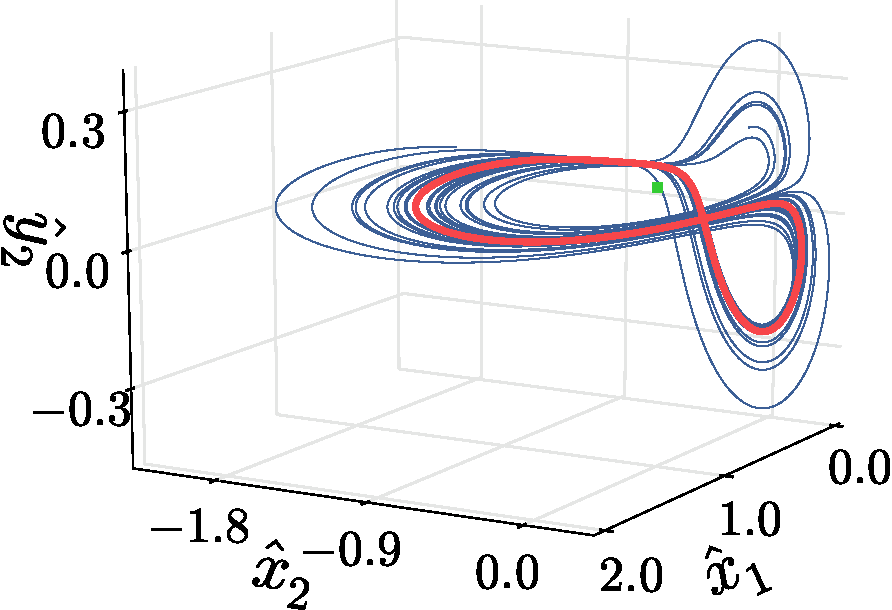
\includegraphics[width=0.21\textwidth]{2modes-sspRed} %\\
%  \quad (a) & \quad (b) & \quad (c) & (d) & (e) & (f)
%  \end{tabular}
% (d) 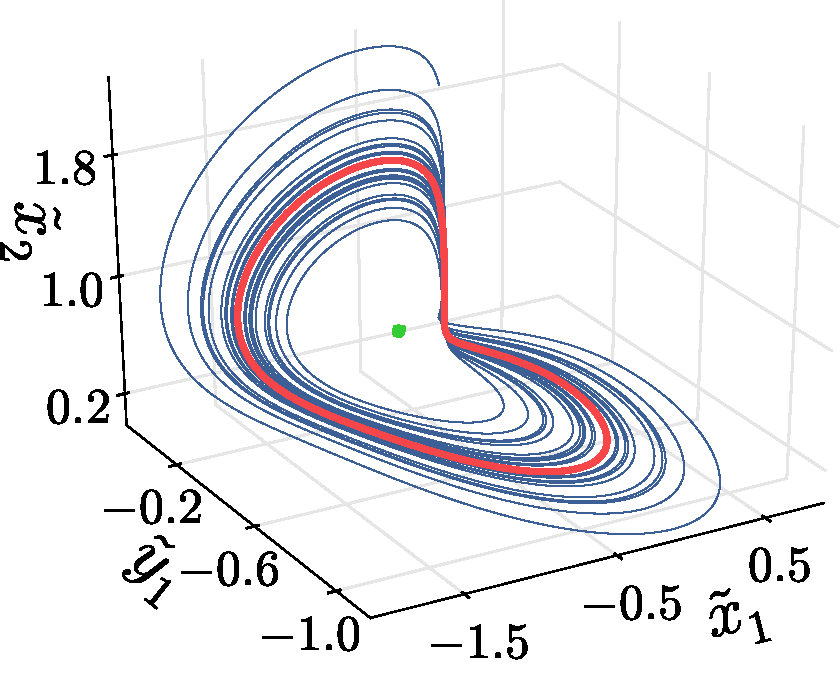
\includegraphics[width=0.20\textwidth]{2modes-sspRed2}
% (d) 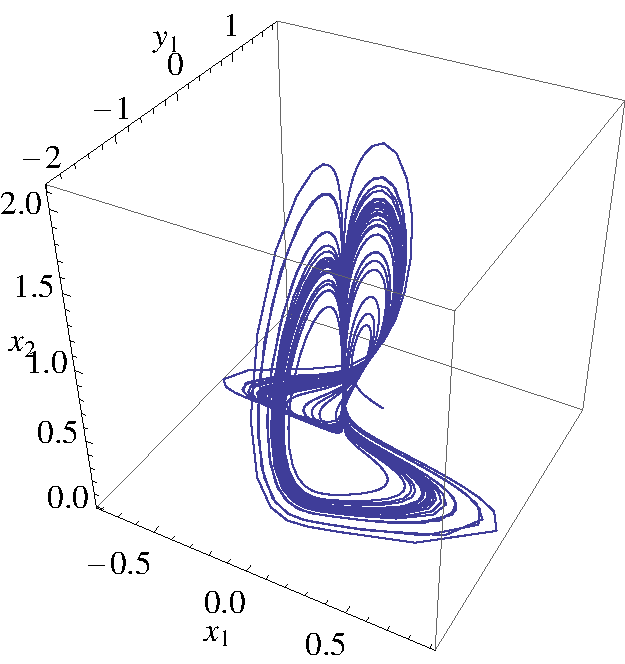
\includegraphics[width=0.20\textwidth]{2modesSliceIntFM2}
\caption{(Color online) 
The \reqv\ (a), two repeats of \rpo\ \cycle{01} (b), and a typical
ergodic trajectory of the \twomode\ system in the configuration
space; same trajectories colored green, red and blue respectively 
in a 3D projection of four-dimensional \statesp\ (d), invariant 
polynomials (e), and the first Fourier mode \slicePlane\ (f).}
\label{fig:Set1}
\end{figure}
\ES{2014-05-15}{I have replaced the second-mode slice, double-angled figure in \reffig{fig:Set1}(b)
with one resulting by integrating on the $(0,0,1,0)$ slice, for consistency with
panel (c). I hope Burak will replace it with a publication quality figure of the same
representation. The trick of angle doubling will be introduced in its own section.
}
\begin{table}
	\caption{Parameters used here to study the \twomode\ system.}
	\begin{tabular}{c|c|c|c|c|c|c|c|c|c}
	% after \\: \hline or \cline{col1-col2} \cline{col3-col4} ...
	 $\mu_1$ & $\mu_2$ & $e_1$ & $e_2$ & $a_1$ & $a_2$ & $b_1$ & $b_2$ & $c_1$ & $c_2$ \\
	\hline   
	 -2.8	& 1		  & 0	  & 1	  & -1	  & -2.66 & 0	  & 0 	  & -7.75 & 1	  \\
	\end{tabular}
	\label{tab:pars}
\end{table}
To illustrate the \mslices\ on the \twomode\ system we choose a simple 
set of parameters for which we observe interesting dynamics. These
parameters are listed in \reftab{tab:pars}. With this set of parameters,
we can write \twomode\ ODEs \refeq{eq:DangSO2} in terms of three parameters $\{ \mu_1, c_2, a_2 \}$:
\bea
\label{eq:DangSO2set1}
  \sspC_1 &=& \mu_1 \,z_1 - z_1|z_1|^2 +c_1\,\overline{z}_1\,z_2
  \continue
  \sspC_1 &=& (1-\ii)\,{z_2}+a_2\,z_2|z_1|^2+\,z_1^2
\,,
\eea
Note that by setting $b_2 = 0$, we send the \reqv\ at $\invpol = (0,-\mu_2/b_2,0,0)$ to infinity. Moreover, \refeq{PKinvEqs5a} yields $\tilde{v} = (\mu_1 + \tilde{a}_1 \tilde{u})/(\mu_2 + \tilde{a}_2 \tilde{u} - \tilde{u} \tilde{b}_1)$. Substitution into \refeq{PKinvEqs5b} allows one to solve for a single variable. By solving \refeq{PKinvEqs5} with the parameter set \reftab{tab:pars},
we get two real roots, with non-negative $u$ and $v$: %the \eqva\ of the system in the invariant polynomial basis \refeq{Dang86(1.2)PK} as
\[
	\invpol_{\EQV{}} = (0,0,0,0)^T %\qquad \mbox{(double)}
\]
which is a double root and corresponds to an equilibrium of \refeq{eq:DangSO2}, and
\[
			 \invpol_{\REQV{}{}} = (0.193569,0.154131,-0.149539,-0.027178)^T\,,
\]
which is a relative equilibrium. In real representation, a
representative point on  \REQV{}{} may be chosen as
\[
  \left(x_1, y_1, x_2, y_2\right) = \left(0.439966, 0, -0.386267, 0.070204\right)
\]
We visualize the dynamics of the \twomode\ system in four different representations: 3D projections of the four-dimensional real valued \statesp and invariant polynomials, in the 3D \slicePlane\ and on the 2D configuration space plots on which the color-coded field $u(\conf, \zeit)$ is defined as follows:
\bea
	u(\conf, \tau) &=& \sum_{k=-2}^{2} \sspC_k(\zeit) e^{i k \conf}\, ,
	\continue && \mbox{where} \, \sspC_{-k} = \sspC_k^* \, \mbox{and} \,
	\sspC_0 = 0 \, .
\eea
\refFig{fig:Set1} shows the only \reqv , \rpo\ \cycle{01} and an ergodic trajectory of the \twomode\ system in the four different representations we described above. Note that translation of the \reqv\ in the configuration space \reffig{fig:Set1} (a), corresponds to the \SOn{2} rotations in the \statesp\ of Fourier modes in \reffig{fig:Set1} (d) (green curve) and these orbits correspond to a single point in the symmetry reduced representations of \reffig{fig:Set1} (e, f). Note also that the \rpo\ \cycle{01} translates/rotates as it advances in configuration space (\reffig{fig:Set1} (b)) and in the equivariant \statesp\ \reffig{fig:Set1} (\reffig{fig:Set1} (d)), whereas in the symmetry reduced plots (\reffig{fig:Set1} (e, f)), it closes onto itself after one period.

The simple structure of the symmetry reduced dynamics allows us to determine the 
\rpo s of the \twomode\ system by means of a Poincar\'e section and a return map. We illustrated this procedure in \reffig{fig:psectandretmap}. Starting with an initial
point close to the \REQV{}{}, we computed a long ergodic trajectory of the symmetry reduced \twomode\ system by integrating \refeq{e-so2red1stmode} (blue curve in \reffig{fig:psectandretmap} (a)) and recorded its intersections (marked with red in \reffig{fig:psectandretmap} (a)) with the Poincar\'e section (transparent plane in \reffig{fig:psectandretmap} (a)), which includes the \REQV{}{} and the imaginary part of its unstable stability eigenvector (one of the green arrows in \reffig{fig:psectandretmap} (a)). We then projected these intersections onto a
basis $(v_1, v_2)$, which spans the Poincar\'e section, and fit cubic splines to this set of points, see \reffig{fig:psectandretmap} (b). The return map of arclengths from the origin which is set to \REQV{}{} in \reffig{fig:psectandretmap} (b), is unimodal with an sharp cusp located at its critical point, shown in \reffig{fig:psectandretmap} (c). Note that the region corresponds to the neighborhood of the \reqv\ $s = (0, 0.6)$ is never visited once the flow leaves this region and falls onto the chaotic attractor. For this reason, we re-drew this return map after discarding the data corresponding to the initial transients in \reffig{fig:psectandretmap} (d). We use this return map to determine the accessible \rpo s  with their respective binary symbol sequences.

\begin{figure}
\centering
  (a) 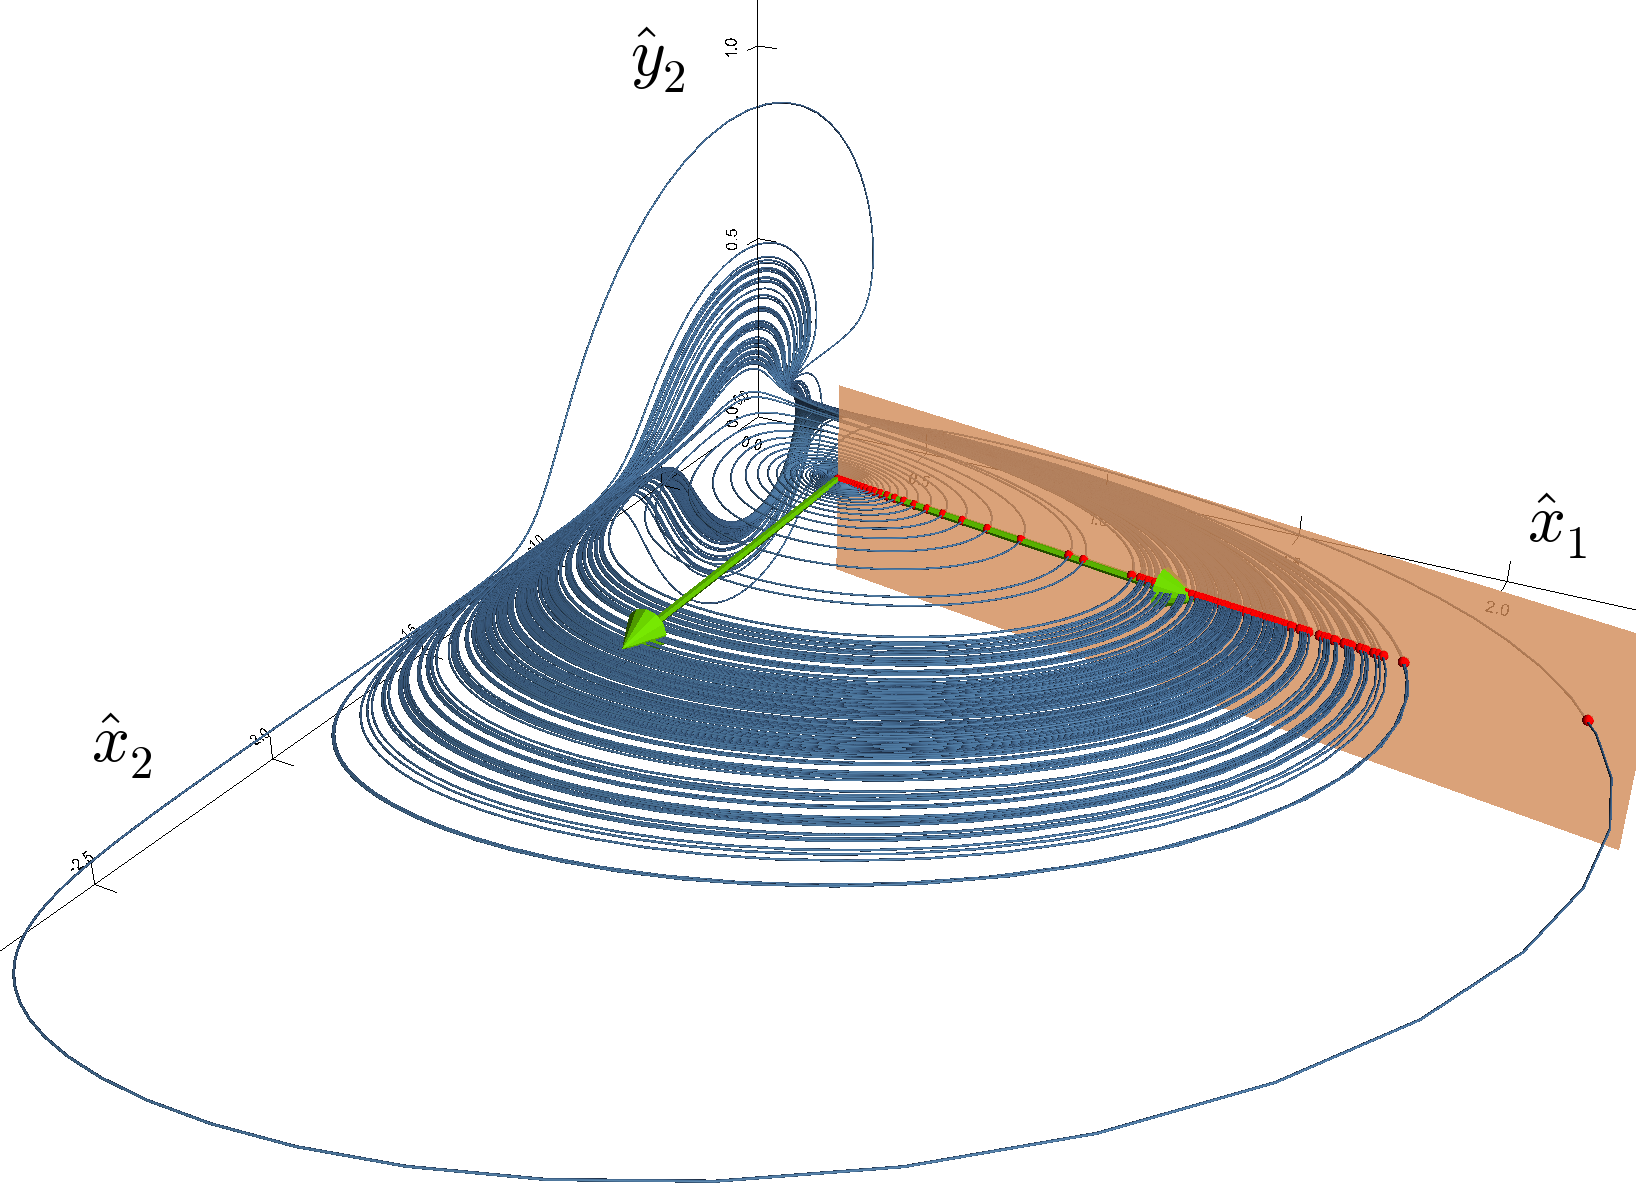
\includegraphics[width=0.45\textwidth]{BBpsecthd} \\
  (b) 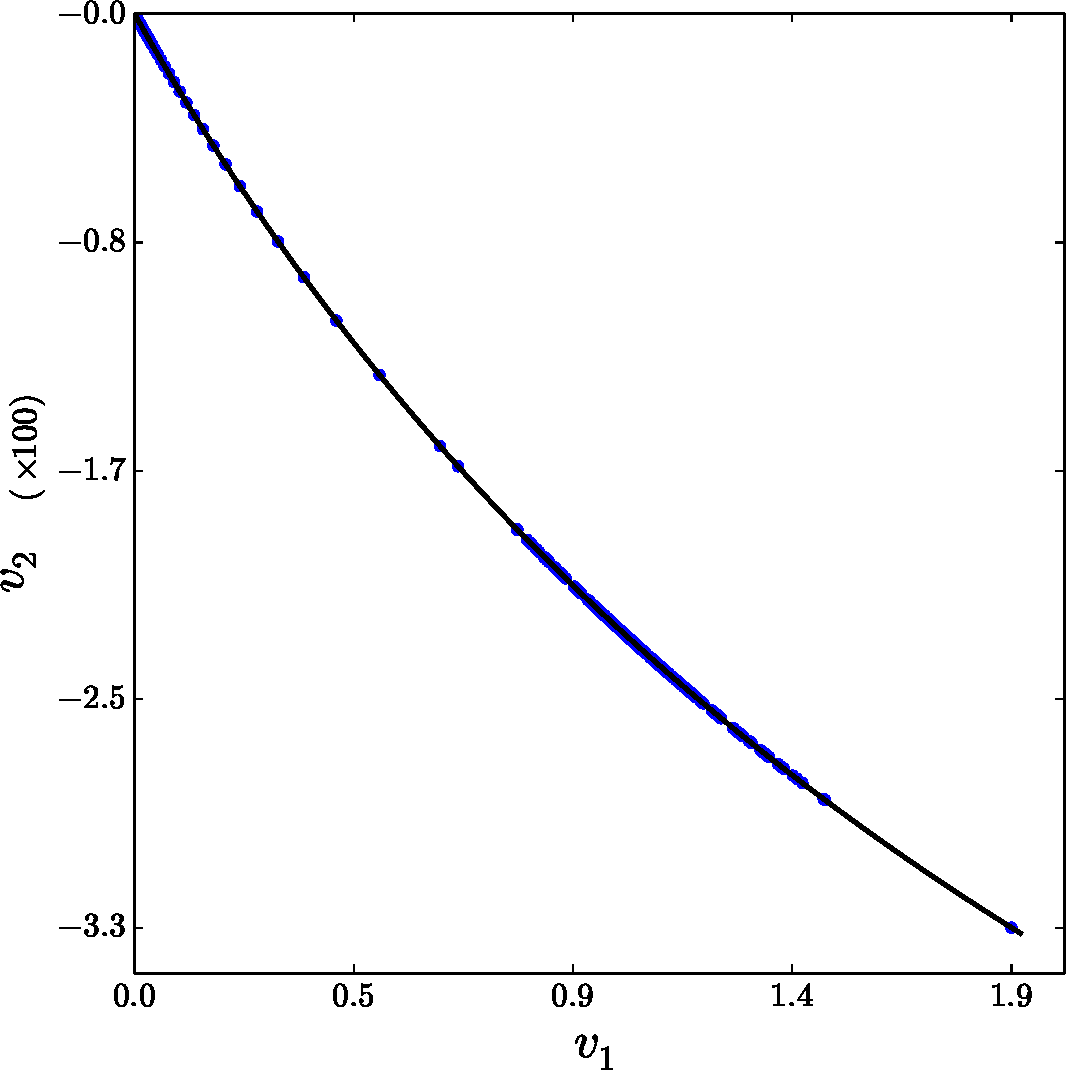
\includegraphics[width=0.20\textwidth]{BBpsectonslice}
  (c) 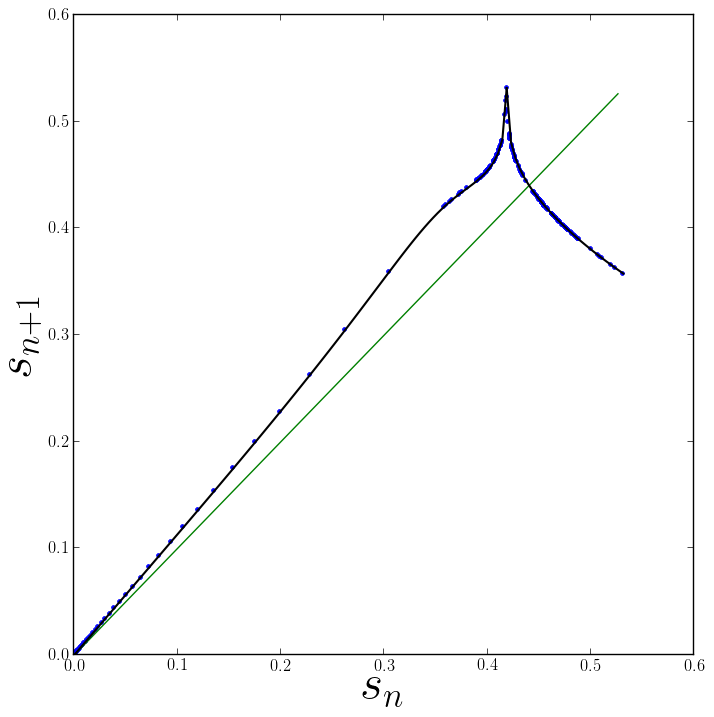
\includegraphics[width=0.20\textwidth]{BBretmaponslice} \\
  (d) 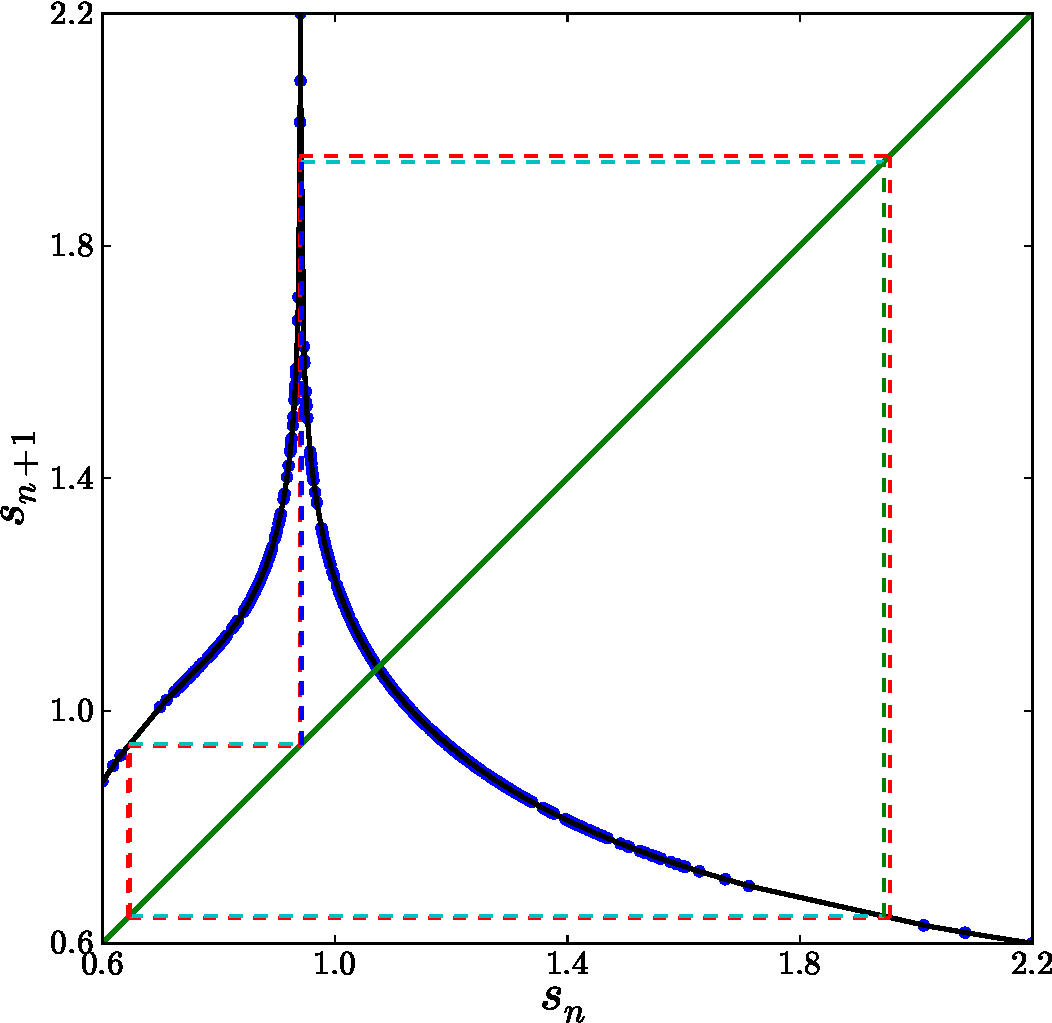
\includegraphics[width=0.45\textwidth]{BBretmaponsliceZoom}
\caption{(a) Symmetry reduced flow within the slice hyperplane (blue).
			Green arrows show the real and imaginary part of the unstable stability
			eigenvector $v_u$ of \REQV{}{}. A Poincar\'e section which includes
			$Im[v_u]$ is visualized as a transparent plane, and sections
			of the flow by the Poincar\'e section are marked with red.
		 (b) The Poincar\'e section which includes the \REQV{}{} and $v_u$ projected
			on to the basis within the plane shown in (a). Included is a
            transient trajectory initiated close to \REQV{}{}. Note that
		  	the vertical axis is magnified by $100$.
		 (c) The Poincar\'e arclength return map for the
		    Poincar\'e section (b).
		 (d) The return map without the transient points, framed by
            orbit of the critical point.
		 	Dashed lines show the 3-cycle \cycle{001}.}
\label{fig:psectandretmap}
\end{figure}